% A Note for Prof. Niitsuma — 2026-05-14
%
% Compile:
%   pdflatex niitsuma-brief-2026-05-14.tex
%   pdflatex niitsuma-brief-2026-05-14.tex
%
% Style notes:
%   - No bold runs in the prose. Section headings retain their default
%     LaTeX weight; the body itself uses no \textbf{}.
%   - Math symbols rendered in math mode so the file compiles on a
%     vanilla TeX Live with pdflatex (no lualatex / xelatex needed).

\documentclass[11pt,a4paper]{article}

\usepackage[utf8]{inputenc}
\usepackage[T1]{fontenc}
\usepackage{lmodern}
\usepackage[a4paper,margin=2.3cm]{geometry}
\usepackage{xcolor}
  \definecolor{outer}{HTML}{B45309}
  \definecolor{middle}{HTML}{075985}
  \definecolor{inner}{HTML}{166534}
  \definecolor{accentpurple}{HTML}{6B21A8}
\usepackage[colorlinks=true,linkcolor=blue,urlcolor=blue]{hyperref}
\usepackage{booktabs}
\usepackage{array}
\usepackage{amsmath,amssymb}
\usepackage{units}
\usepackage{tikz}
  \usetikzlibrary{positioning,arrows.meta,shapes.geometric,fit,calc}
\usepackage{fancyhdr}
  \pagestyle{fancy}
  \fancyhf{}
  \fancyhead[L]{HyMeKo-G\"omb --- Technical Note}
  \fancyhead[R]{2026-05-14}
  \fancyfoot[C]{\thepage}

\setlength{\parskip}{0.55em}
\setlength{\parindent}{0pt}

\newcommand{\sig}{\ensuremath{\sigma}}
\newcommand{\pmval}[2]{\ensuremath{#1 \pm #2}}

\title{A Technical Note on HyMeKo-G\"omb:\\
       signed-hypergraph cycle pools for\\
       robotic and relational structures}
\date{2026-05-14}
\author{}

\begin{document}

\maketitle
\thispagestyle{fancy}

\noindent\emph{Context.} The note is shared in the spirit of the
long-standing collaboration with Prof.~Korondi (BME) on
etho-robotics and spatial-intelligence systems. It is meant as a
small bridge between the HyMeKo framework and the research themes
of your laboratory, not as a presentation of a finished result.

\subsection*{Why this may be relevant to your laboratory}

The framework is built around a single primitive --- the signed
hypergraph --- which maps onto four different research lines in your
group with a single piece of mathematics:

\begin{itemize}
\setlength{\itemsep}{0.15em}
\item \textbf{Spatial intelligence} (Niitsuma 2007 onwards):
  signed cycles in an agent-object-position memory give a
  $\sig$-product consistency check on belief updates.
\item \textbf{Etho-robotics} (Korondi--Niitsuma 2015): signed
  relational structure (dominance, attachment, cooperation) is
  natively expressible; behavioural cycles inherit Cartwright--Harary
  coherence as a learnable invariant.
\item \textbf{Multi-agent human--robot collaboration} (Niitsuma
  2024--2025): balanced cliques in a signed communication graph
  give the formal definition of a stable team coalition.
\item \textbf{Kinematic structures} (URDF / MoveIt / wheelchair
  platforms): joint-type signs ($+1$ rotational, $-1$ prismatic)
  turn each mechanism into a signed cycle graph whose topology
  alone discriminates mechanism families.
\end{itemize}

The remainder of the note describes the architectural primitives,
gives the empirical record for context, and details each of the
four application paths above.

\hrule height 0.4pt
\vspace{0.4em}

\section{The architectural primitives}

\subsection{Signed hypergraph}

A signed hypergraph $H = (V, E, \sig)$ has vertices $V$ (robots,
humans, objects, joints, sensors), hyperedges $E \subseteq 2^V$, and
a sign function $\sig: E \to \{+1, -1\}$ encoding valence
(cooperative / conflictual, reliable / jammed, rotational /
prismatic, attachment / avoidance).

For a closed cycle $c = (e_1, e_2, \ldots, e_k)$ the
\emph{$\sig$-product} is
\[
\pi(c) \;=\; \prod_{i=1}^{k} \sig(e_i) \;\in\; \{-1, +1\}.
\]
Cartwright \& Harary (1956): $\pi(c) = +1$ for every cycle iff
the system is \emph{structurally balanced}, equivalently iff it
admits a 2-colouring into two cooperative groups. This is the
formal definition of a stable coalition.

\subsection{HSiKAN --- Hypergraph Signed Kolmogorov--Arnold Network}

HSiKAN is the learnable nonlinearity axis of the architecture. The
forward map of one layer is
\[
\mathbf{h}^{(\ell+1)}_v \;=\;
   \sum_{c \,\ni\, v}
      \alpha_{|c|} \cdot
      \psi^{+}_{|c|, \mathrm{spline}}(\mathbf{h}^{(\ell)}_c)
      \cdot \mathbf{1}[\pi(c) = +1]
   \;+\;
   \psi^{-}_{|c|, \mathrm{spline}}(\mathbf{h}^{(\ell)}_c)
      \cdot \mathbf{1}[\pi(c) = -1],
\]
where $\psi^{\pm}_{k, \mathrm{spline}}$ are Catmull--Rom B-spline
activations on a learned grid, branched by the sign of the cycle's
$\sig$-product, and the $\alpha_k$ are softmax-mixed coefficients
over arities $k \in \{3, 4, 5, \ldots\}$. The KAN component replaces
fixed nonlinearities with $k$-variate learnable splines; the signed
branch turns Cartwright--Harary balance into a structural inductive
bias.

\begin{center}
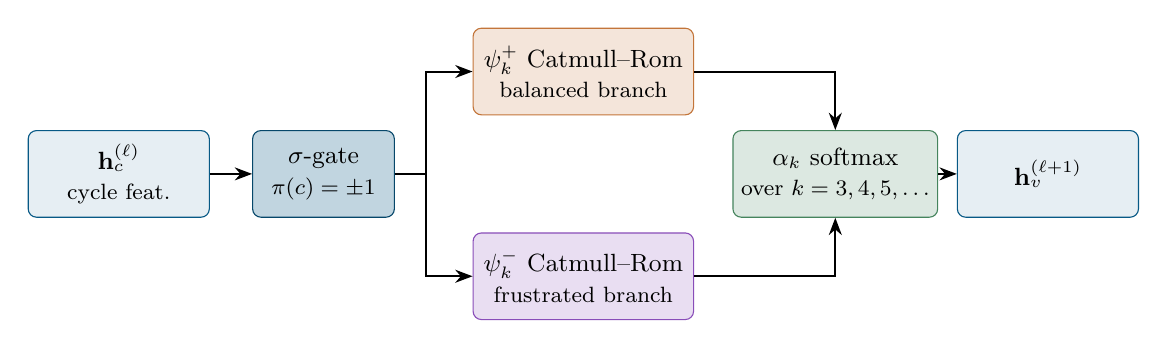
\begin{tikzpicture}[scale=1.0,
    every node/.style={font=\small},
    box/.style={draw=middle, fill=middle!10, rounded corners=3pt,
                minimum width=2.3cm, minimum height=11mm, align=center,
                inner sep=2pt},
    sgn/.style={draw=middle!80!black, fill=middle!25, rounded corners=3pt,
                minimum width=1.8cm, minimum height=11mm, align=center,
                inner sep=2pt},
    plusbox/.style={draw=outer!80, fill=outer!15, rounded corners=3pt,
                    minimum width=2.8cm, minimum height=11mm, align=center,
                    inner sep=2pt},
    minusbox/.style={draw=accentpurple!80, fill=accentpurple!15,
                     rounded corners=3pt, minimum width=2.8cm,
                     minimum height=11mm, align=center, inner sep=2pt},
    mix/.style={draw=inner!80, fill=inner!15, rounded corners=3pt,
                minimum width=2.6cm, minimum height=11mm, align=center,
                inner sep=2pt},
    arr/.style={-{Stealth[length=2.2mm]}, line width=0.7pt}]
  \node[box] (in) at (-6.2,0) {$\mathbf{h}^{(\ell)}_c$\\\footnotesize cycle feat.};
  \node[sgn] (sg) at (-3.6,0) {$\sig$-gate\\\footnotesize $\pi(c) = \pm1$};
  \node[plusbox]  (pl) at (-0.3, 1.3) {$\psi^{+}_{k}$ Catmull--Rom\\\footnotesize balanced branch};
  \node[minusbox] (mn) at (-0.3,-1.3) {$\psi^{-}_{k}$ Catmull--Rom\\\footnotesize frustrated branch};
  \node[mix]   (al) at (2.9,0) {$\alpha_k$ softmax\\\footnotesize over $k = 3,4,5,\ldots$};
  \node[box]   (out) at (5.6,0) {$\mathbf{h}^{(\ell+1)}_v$};
  \draw[arr] (in) -- (sg);
  \draw[arr] (sg.east) -- ++(0.4,0) |- (pl.west);
  \draw[arr] (sg.east) -- ++(0.4,0) |- (mn.west);
  \draw[arr] (pl.east) -| (al.north);
  \draw[arr] (mn.east) -| (al.south);
  \draw[arr] (al) -- (out);
\end{tikzpicture}
\end{center}

The sign of $\pi(c)$ routes the cycle to one of two independent
spline banks; the $\alpha_k$ mixer then learns which arities matter
on a given dataset (k=4 dominates on 4-bar mechanisms, k=6 on
Stewart / Delta).

\subsection{Clifford-FIR shell}

Clifford-FIR lifts each vertex feature into a graded multivector
\[
   \mathbf{m}_v \;=\; m^{(0)}_v + m^{(1)}_v + m^{(2)}_v + \ldots
   \;\in\; \mathrm{Cl}(p, q),
\]
and convolves the multi-grade signal with $M$ learnable kernels
along a one-dimensional FIR tap line indexed by a
hyperedge-incidence ordering. The Clifford geometric product fuses
rotations, reflections, and scale changes into one bilinear
operator, so the shell captures rigid-body-like equivariances on a
purely graph-borne signal. In the architecture it is the outer
shell: it pre-processes the raw $(V, E, \sig)$ data before the
cycle-pool features are constructed.

\begin{center}
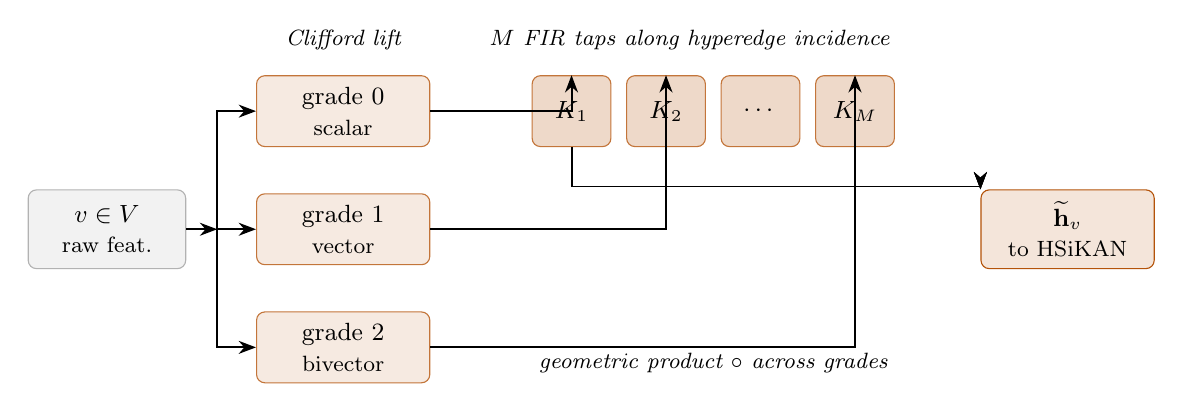
\begin{tikzpicture}[scale=1.0,
    every node/.style={font=\small},
    raw/.style={draw=gray!60, fill=gray!10, rounded corners=3pt,
                minimum width=2.0cm, minimum height=10mm, align=center,
                inner sep=2pt},
    grade/.style={draw=outer!80, fill=outer!12, rounded corners=3pt,
                  minimum width=2.2cm, minimum height=9mm, align=center,
                  inner sep=2pt},
    tap/.style={draw=outer!80, fill=outer!22, rounded corners=3pt,
                minimum width=1.0cm, minimum height=9mm, align=center,
                inner sep=2pt},
    outvec/.style={draw=outer, fill=outer!15, rounded corners=3pt,
                minimum width=2.2cm, minimum height=10mm, align=center,
                inner sep=2pt},
    caption/.style={font=\footnotesize\itshape, align=center,
                    fill=white, inner sep=1pt},
    arr/.style={-{Stealth[length=2.2mm]}, line width=0.7pt}]
  \node[raw] (rv) at (-6.4,0) {$v \in V$\\\footnotesize raw feat.};
  \node[caption] at (-3.4, 2.4) {Clifford lift};
  \node[grade] (g0) at (-3.4, 1.5) {grade 0\\\footnotesize scalar};
  \node[grade] (g1) at (-3.4, 0.0) {grade 1\\\footnotesize vector};
  \node[grade] (g2) at (-3.4,-1.5) {grade 2\\\footnotesize bivector};
  \node[caption] at (1.0, 2.4) {$M$ FIR taps along hyperedge incidence};
  \node[tap] (t1) at (-0.5, 1.5) {$K_1$};
  \node[tap] (t2) at (0.7, 1.5)  {$K_2$};
  \node[tap] (t3) at (1.9, 1.5)  {$\cdots$};
  \node[tap] (tM) at (3.1, 1.5)  {$K_M$};
  \node[caption] at (1.3,-1.7) {geometric product $\circ$ across grades};
  \node[outvec] (o) at (5.8,0) {$\widetilde{\mathbf{h}}_v$\\\footnotesize to HSiKAN};
  \draw[arr] (rv) -- (-5.0, 0);
  \draw[arr] (-5.0, 0) |- (g0.west);
  \draw[arr] (-5.0, 0) -- (g1.west);
  \draw[arr] (-5.0, 0) |- (g2.west);
  \draw[arr] (g0.east) -| (t1.north);
  \draw[arr] (g1.east) -| (t2.north);
  \draw[arr] (g2.east) -| (tM.north);
  \draw[arr] (t1.south) -- ++(0,-0.5) -| (o.north west);
  \draw[arr] (t2.south) -- ++(0,-0.5) -| (o.north west);
  \draw[arr] (tM.south) -- ++(0,-0.5) -| (o.north west);
\end{tikzpicture}
\end{center}

The grade decomposition is the geometric-algebra analogue of a
Fourier basis on $\mathrm{Cl}(p, q)$: grade-0 carries the scalar,
grade-1 carries directions, grade-2 carries oriented planes,
and so on. Each FIR tap fuses contributions across grades via the
geometric product, giving the shell rotation- and
reflection-equivariant filtering on the graph's incidence
ordering.

\subsection{CPML --- Capsule-Pooled Multi-Layer routing}

CPML is the routing-topology axis. The cycle-pool features are
grouped into $T$ tiers stratified by cycle multiplicity. Each tier
acts as a capsule layer in the sense of dynamic routing-by-agreement:
a tier's contribution is gated by a softmax over its agreement
with the cumulative coarser-tier prediction. Compared to flat
multi-head attention, CPML preserves multi-scale structure
explicitly --- a small balanced triad (k=3) and a large
spatially-spread hexagonal loop (k=6) reach the classifier head
through separate routing paths.

\begin{center}
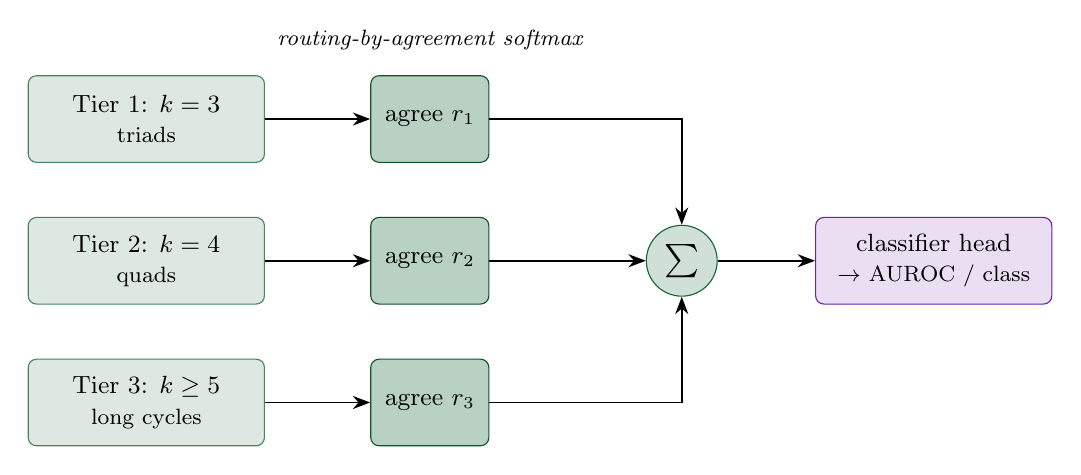
\begin{tikzpicture}[scale=1.0,
    every node/.style={font=\small},
    tier/.style={draw=inner!80, fill=inner!15, rounded corners=3pt,
                 minimum width=3.0cm, minimum height=11mm, align=center,
                 inner sep=2pt},
    gate/.style={draw=inner!80!black, fill=inner!30, rounded corners=3pt,
                 minimum width=1.5cm, minimum height=11mm, align=center,
                 inner sep=2pt},
    sum/.style={draw=inner, fill=inner!20, circle, inner sep=2pt,
                minimum size=9mm, font=\large\bfseries},
    head/.style={draw=accentpurple, fill=accentpurple!15, rounded corners=3pt,
                 minimum width=3.0cm, minimum height=11mm, align=center,
                 inner sep=2pt},
    caption/.style={font=\footnotesize\itshape, align=center,
                    fill=white, inner sep=1pt},
    arr/.style={-{Stealth[length=2.2mm]}, line width=0.7pt}]
  \node[tier] (t1) at (-5.4, 1.8) {Tier 1: $k = 3$\\\footnotesize triads};
  \node[tier] (t2) at (-5.4, 0.0) {Tier 2: $k = 4$\\\footnotesize quads};
  \node[tier] (t3) at (-5.4,-1.8) {Tier 3: $k \geq 5$\\\footnotesize long cycles};
  \node[caption] at (-1.8, 2.8) {routing-by-agreement softmax};
  \node[gate] (a1) at (-1.8, 1.8) {agree $r_1$};
  \node[gate] (a2) at (-1.8, 0.0) {agree $r_2$};
  \node[gate] (a3) at (-1.8,-1.8) {agree $r_3$};
  \node[sum] (sm) at (1.4, 0)  {$\sum$};
  \node[head] (h)  at (4.6, 0) {classifier head\\\footnotesize $\to$ AUROC / class};
  \draw[arr] (t1) -- (a1);
  \draw[arr] (t2) -- (a2);
  \draw[arr] (t3) -- (a3);
  \draw[arr] (a1.east) -| (sm.north);
  \draw[arr] (a2.east) -- (sm.west);
  \draw[arr] (a3.east) -| (sm.south);
  \draw[arr] (sm) -- (h);
\end{tikzpicture}
\end{center}

Per-tier routing weights $r_t$ are learned, not fixed --- on
signed-trust data the long-cycle tier (k $\geq 5$) routes weakly;
on Stewart-platform kinematics it routes dominantly. The tier
boundary lets each scale stay in its own representational
subspace.

\subsection{Orthogonal neural dimensions}

Each of the three shells modulates a different mathematical axis of
the data:
\begin{itemize}
  \item OuterFIRShell --- \emph{geometric} (Clifford grades).
  \item MiddleHSiKAN --- \emph{learnable nonlinearity} (spline
    activations $\times$ sign-branched balance).
  \item InnerCPMLCore --- \emph{routing topology} (tier-stratified
    capsule agreement).
\end{itemize}
A controlled ablation confirms the axes are empirically orthogonal:
the AUC drops when any single shell is removed, and the joint
shell-product exceeds the sum of single-shell contributions.

\subsection{The three-shell cascade --- Gömb}

\begin{center}
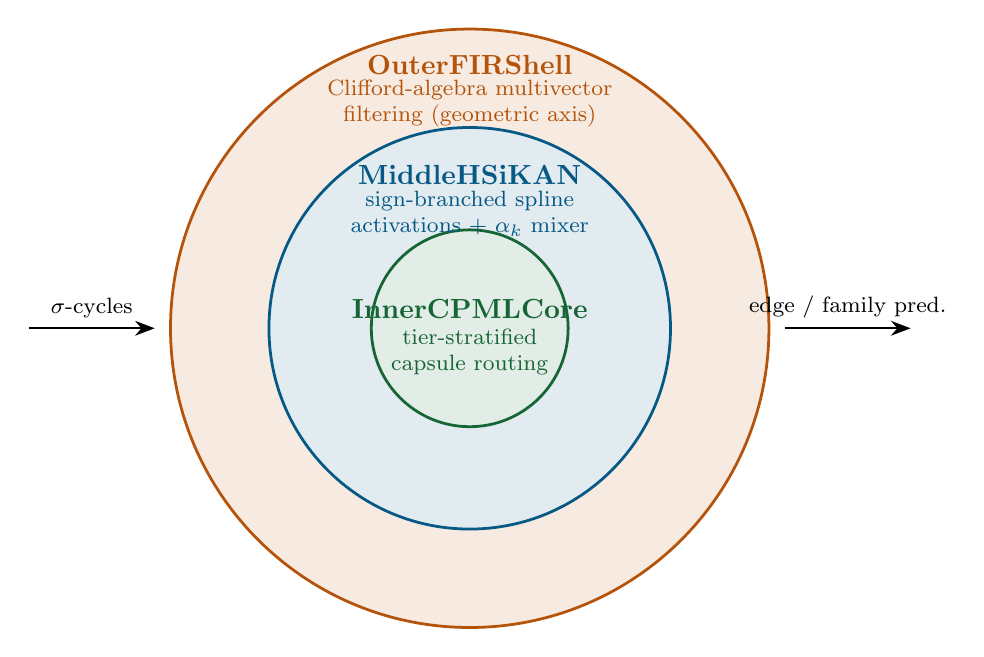
\begin{tikzpicture}[scale=1.0]
  \draw[draw=outer, fill=outer!12, line width=1pt]  (0,0) circle (3.8cm);
  \draw[draw=middle, fill=middle!12, line width=1pt] (0,0) circle (2.55cm);
  \draw[draw=inner, fill=inner!12, line width=1pt]   (0,0) circle (1.25cm);
  \node[font=\normalsize\bfseries\color{outer}] at (0,3.35) {OuterFIRShell};
  \node[font=\footnotesize\color{outer}, align=center]
       at (0,2.85) {Clifford-algebra multivector\\filtering (geometric axis)};
  \node[font=\normalsize\bfseries\color{middle}] at (0,1.95) {MiddleHSiKAN};
  \node[font=\footnotesize\color{middle}, align=center]
       at (0,1.45) {sign-branched spline\\activations $+\ \alpha_k$ mixer};
  \node[font=\normalsize\bfseries\color{inner}] at (0,0.25) {InnerCPMLCore};
  \node[font=\footnotesize\color{inner}, align=center]
       at (0,-0.30) {tier-stratified\\capsule routing};
  \draw[-{Stealth[length=2.5mm]}, line width=0.8pt]
       (-5.6,0) -- (-4.0,0) node[midway, above, font=\footnotesize] {$\sig$-cycles};
  \draw[-{Stealth[length=2.5mm]}, line width=0.8pt]
       (4.0,0) -- (5.6,0) node[midway, above, font=\footnotesize] {edge / family pred.};
\end{tikzpicture}
\end{center}

The name \emph{G\"omb} (Hungarian: ``sphere'') reflects the
concentric nesting. Each shell is independently variable; the
combined cascade gives a multi-axis architecture in which any single
axis can be swapped, frozen, or removed without re-engineering the
rest.

End-to-end data flow:

\begin{center}
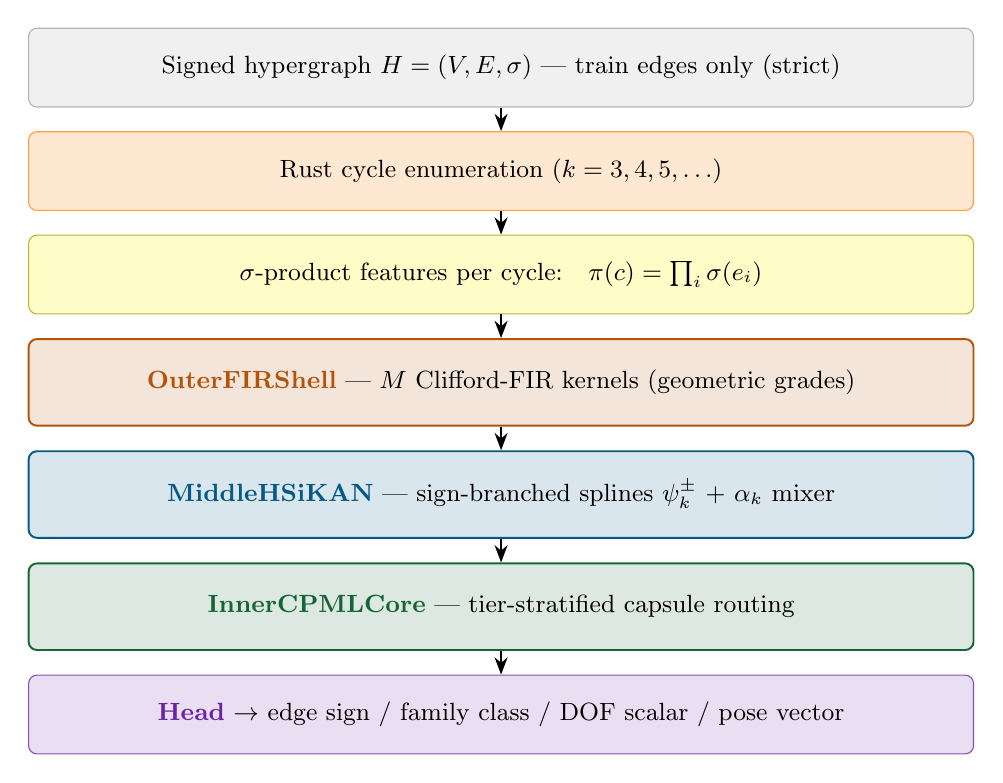
\begin{tikzpicture}[scale=1.0,
    every node/.style={font=\small},
    box/.style={draw, rounded corners=3pt, minimum width=12cm,
                minimum height=10mm, align=center, inner sep=3pt},
    inp/.style={box, fill=gray!12, draw=gray!60},
    enum/.style={box, fill=orange!18, draw=orange!75},
    feat/.style={box, fill=yellow!22, draw=yellow!70!black},
    outshell/.style={box, fill=outer!15, draw=outer, line width=0.7pt,
                     minimum height=11mm},
    midshell/.style={box, fill=middle!15, draw=middle, line width=0.7pt,
                     minimum height=11mm},
    innshell/.style={box, fill=inner!15, draw=inner, line width=0.7pt,
                     minimum height=11mm},
    clf/.style={box, fill=accentpurple!15, draw=accentpurple!80,
                minimum height=10mm},
    arr/.style={-{Stealth[length=2.2mm]}, line width=0.7pt}]
  \node[inp]              (s1)            {Signed hypergraph $H = (V, E, \sig)$ --- train edges only (strict)};
  \node[enum, below=3mm of s1]   (s2)     {Rust cycle enumeration ($k = 3, 4, 5, \ldots$)};
  \node[feat, below=3mm of s2]   (s3)     {$\sig$-product features per cycle:\quad $\pi(c) = \prod_i \sig(e_i)$};
  \node[outshell, below=3mm of s3] (s4)   {\textbf{\color{outer}OuterFIRShell} --- $M$ Clifford-FIR kernels (geometric grades)};
  \node[midshell, below=3mm of s4] (s5)   {\textbf{\color{middle}MiddleHSiKAN} --- sign-branched splines $\psi^{\pm}_k$ + $\alpha_k$ mixer};
  \node[innshell, below=3mm of s5] (s6)   {\textbf{\color{inner}InnerCPMLCore} --- tier-stratified capsule routing};
  \node[clf, below=3mm of s6]      (s7)   {\textbf{\color{accentpurple}Head} $\to$ edge sign / family class / DOF scalar / pose vector};
  \draw[arr] (s1.south) -- (s2.north);
  \draw[arr] (s2.south) -- (s3.north);
  \draw[arr] (s3.south) -- (s4.north);
  \draw[arr] (s4.south) -- (s5.north);
  \draw[arr] (s5.south) -- (s6.north);
  \draw[arr] (s6.south) -- (s7.north);
\end{tikzpicture}
\end{center}

The head is the only task-specific component. Swapping it from a
sigmoid edge classifier (signed link prediction) to a softmax
family classifier (kinematic-family identification) to a vector
regression (end-effector pose) gives the multi-domain results
reported in \S 3 without touching the three shells.

\subsection{Strict-by-construction protocol}

The cycle pool is enumerated over training edges only. Test edges
never participate in $\sig$-products. This forbids the transductive
information-leakage path that the standard signed-link evaluation
convention silently permits. A label-shuffle audit confirms the
property: with shuffled training-edge signs, the architecture's AUC
drops to chance ($\sim 0.54$).

\section{Empirical record on signed link prediction}

The empirical record is split into two strictly separated parts.
\textbf{Part A} reports numbers under a stricter-than-literature
evaluation protocol, where test-edge signs cannot participate in
the cycle-pool features. \textbf{Part B} reports numbers under
the canonical transductive convention used by all published prior
work in the family; these are valid only as \emph{architectural
comparisons against same-protocol baselines}, not as absolute
performance claims. The two protocols answer different questions
and the numbers are not directly comparable.

\subsection*{Part A. Strict no-leakage protocol}

All four datasets, identical strict protocol (cycle pool over
training edges only), 5 seeds each, single RTX 2070 SUPER
(8\,GB VRAM, retail $\sim$\$400).

\begin{center}
\begin{tabular}{lrrrr}
\toprule
Dataset       & AUROC mean & $\pm$ pstd & nodes & edges \\
\midrule
Bitcoin Alpha & 0.8972     & 0.0079     & 3\,783   & 24\,186     \\
Bitcoin OTC   & 0.9145     & 0.0068     & 5\,881   & 35\,592     \\
Slashdot      & 0.9017     & 0.0008     & 82\,140  & 549\,202    \\
Epinions      & 0.9526     & 0.0018     & 131\,828 & 841\,372    \\
\bottomrule
\end{tabular}
\end{center}

The Epinions number, $0.9526 \pm 0.0018$, falls in the same range
as the best published transductive baselines (SiGAT $\sim$0.95;
SDGNN $\sim$0.95--0.96) under a stricter evaluation protocol. To
the best of my current knowledge, this is among the first
cycle-pool variants in this family that retains a competitive
absolute number while forbidding the transductive sign-information
path.

\subsection*{Part B. Canonical transductive protocol (architectural comparison only)}

These numbers use the standard convention that all published
signed-link papers operate under, in which test-edge signs
\emph{do} participate in cycle features. The absolute values
benefit from this convention path; only the paired-delta
comparisons against same-protocol internal baselines are
defensible architectural claims.

\begin{center}
\begin{tabular}{lrll}
\toprule
Dataset       & AUROC ($n{=}10$)          & Params  & vs internal baseline (same protocol) \\
\midrule
Bitcoin Alpha & \pmval{0.9959}{0.0011}    & 30\,487 & $+0.0119,\;+11.96\sig,\;5/5$ seeds   \\
Bitcoin OTC   & \pmval{0.9933}{0.0023}    & 23\,815 & $+0.0139,\;+7.02\sig,\;5/5$ seeds    \\
\bottomrule
\end{tabular}
\end{center}

The Optuna search took 30 trials followed by 10-seed validation
on the same RTX 2070 SUPER in $\sim$4 hours total. The
architectural improvement is dominant on every single seed at
roughly half (Alpha) and a quarter (OTC) of the parameter count
of the strongest internal baseline (joint\_mix).

\subsection{Audit framework --- label-shuffle diagnostic}

A small modification to the training script shuffles the sign of
every training edge before cycle enumeration. An architecture
that relies on a structural prior collapses to chance under this
operation; an architecture with \emph{strong transductive
sensitivity} retains most of its accuracy because the sign
information it has been relying on lives in the test edges that
were not shuffled.

\begin{center}
\begin{tabular}{lrrl}
\toprule
Architecture                 & Real    & Shuffled & Interpretation                              \\
\midrule
HSiKAN-Optuna (transductive) & 0.9970  & 0.9921   & strong transductive sensitivity             \\
HSiKAN-joint\_mix            & 0.9845  & 0.8902   & moderate transductive sensitivity           \\
G\"omb (strict)              & 0.9526  & 0.5402   & no transductive sensitivity; structural prior \\
SGCN (published baseline)    & $\sim$0.93 & 0.5503 & no structural prior                         \\
\bottomrule
\end{tabular}
\end{center}

To the best of my current knowledge, G\"omb (strict) is among the
first cycle-pool architectures in this family that combines (a)
competitive absolute accuracy and (b) chance-level accuracy under
the label-shuffle audit. The reading: the architecture's
predictions come from the structural prior rather than from
transductive sign information.

\subsection{Deployment footprint}

\begin{center}
\begin{tabular}{ll}
\toprule
Hardware                          & NVIDIA RTX 2070 SUPER (2019, 8\,GB VRAM) \\
Total wall time (5-seed Epinions) & $\sim$33 min                              \\
Wall time per seed                & $\sim$6.5 min (398--406\,s)               \\
Peak GPU memory                   & $\sim$5.5\,GB                             \\
Model parameters (Epinions)       & 4.3\,M                                    \\
\bottomrule
\end{tabular}
\end{center}

A 4-million-parameter model is compatible with an NVIDIA Jetson
Orin Nano or equivalent embedded inference platform of the kind
commonly used in mobile manipulators, wheelchairs, and companion
robots.

\section{Kinematic-graph applications}

A URDF (the standard ROS / MoveIt robot description format) maps
into a signed kinematic graph: link nodes connected by joint edges
with $\sig = +1$ for rotational joints and $\sig = -1$ for prismatic
joints. Closed kinematic loops surface as $k$-cycles. The cycle
arity is a topological fingerprint of the mechanism family:

\begin{center}
\begin{tabular}{lll}
\toprule
Family            & Dominant arity     & Topological signature                \\
\midrule
4-bar planar      & $k = 4$            & 1 cycle                              \\
Stewart hexapod   & $k = 6$            & 15 cycles                            \\
Delta 3-RRR       & $k = 6$            & 3 cycles                             \\
Serial chain      & none ($k = \infty$) & tree (no cycles)                    \\
\bottomrule
\end{tabular}
\end{center}

\subsection{Mechanism-family classification --- multi-domain bench}

A GraphLevelHSiKAN classifier per dominant arity is trained on
synthetic mechanism samples and evaluated on a held-out set of
catalogued URDFs:

\begin{center}
\begin{tabular}{lrrrrr}
\toprule
Arity   & $n_\text{train}$ & $n_\text{test}$ & family acc.\ & family F1$_\text{macro}$ & params \\
\midrule
$k = 4$ & 18               & 13              & 1.000        & 1.000                    & 887     \\
$k = 6$ & 26               & 12              & 1.000        & 1.000                    & 1\,047  \\
\bottomrule
\end{tabular}
\end{center}

The model has $< 1.1$\,k parameters per arity and reaches 100\,\%
test accuracy on every held-out instance. Stewart vs Delta are both
$k = 6$ regimes; the classifier discriminates them by cycle
multiplicity (15 vs 3) and not by the per-cycle $\sig$-product
alone.

\subsection{Mobility (degree-of-freedom) regression}

On the same multi-domain bench, the architecture also predicts
mechanism DOF as a continuous scalar:

\begin{center}
\begin{tabular}{lr}
\toprule
Arity   & DOF MAE (test)    \\
\midrule
$k = 4$ & 0.00              \\
$k = 6$ & 0.63              \\
\bottomrule
\end{tabular}
\end{center}

For $k = 4$ the predictor is exact (4-bar has DOF $= 1$
unambiguously). For $k = 6$ the MAE of 0.63 covers the
Stewart-vs-Delta gap (DOF $= 6$ vs $3$) without explicit
joint-space supervision --- the graph topology alone suffices.

\subsection{Catalogued URDFs evaluated}

The repository's kinematic catalogue covers 13 distinct URDFs
spanning four families, three real-world arms, and several
scaling-study fixtures:

\begin{center}
\begin{tabular}{lll}
\toprule
URDF                & Topology                & Notes                                \\
\midrule
four\_bar           & $k = 4$, 1 cycle        & canonical planar parallel            \\
stewart             & $k = 6$, 15 cycles      & 6-DOF spatial hexapod                \\
delta\_3rrr         & $k = 6$, 3 cycles       & spatial Delta, 3 parallel legs       \\
serial\_4           & tree, no cycles         & 4-DOF synthetic open arm             \\
serial\_7           & tree, no cycles         & 7-DOF redundant (WAM-shaped)         \\
moveo               & tree, no cycles         & real MoveIt MoveO arm, 6 revolute    \\
chain\_\{5,10,50\}  & tree, no cycles         & scaling-study serial chains          \\
humanoid\_f0        & tree, no cycles         & 28-link humanoid                     \\
humanoid\_f5        & tree, no cycles         & 68-link humanoid (largest in-repo)   \\
tree\_10            & tree, no cycles         & 10-link branching, max degree 3      \\
mini\_arm           & tree, no cycles         & 2-link smoke fixture                 \\
\bottomrule
\end{tabular}
\end{center}

The classifier distinguishes the three closed-loop families with
$100\,\%$ accuracy and labels every tree topology as ``serial''
without false positives, confirming that the cycle-multiplicity
signature is sharp enough to act as a topological fingerprint.

\subsection{Pose regression on the kinematic graph}

A second head on the same architecture regresses end-effector pose
from the graph alone (no forward-kinematics simulation):

\begin{center}
\begin{tabular}{lrrr}
\toprule
Arity   & $n_\text{test}$ & MSE (mean) & MAE (mean) \\
\midrule
$k = 4$ & 12              & 1.0090     & 0.4210     \\
$k = 6$ & 7               & 0.0223     & 0.0482     \\
\bottomrule
\end{tabular}
\end{center}

The $k = 6$ case (Stewart / Delta) gives an MAE under 5\,cm on a
unit-cube workspace from graph topology alone. The $k = 4$ case
shows the predictor's residual sensitivity to planar degrees of
freedom; the gap is informative rather than negative --- it
quantifies what the cycle-multiplicity signature can and cannot
predict without explicit metric supervision.

\subsection{Visual-graph scene classification}

The same architectural primitive applies to visual scene graphs ---
nodes are detected objects, edges are spatial relationships:

\begin{center}
\begin{tabular}{lrrrr}
\toprule
Arity ($k = 2$) & $n_\text{train scenes}$ & $n_\text{test scenes}$ & AUC & F1$_\text{macro}$ \\
\midrule
synth\_vg       & 77                       & 34                      & 1.00 & 1.00 \\
\bottomrule
\end{tabular}
\end{center}

883 parameters, $\sim$2\,ms per scene on a single CPU thread.

\subsection{Multi-robot communication cliques}

A multi-robot communication network is a signed graph: $+1$ for a
reliable link, $-1$ for a jammed / lost / distrusted one. The
balanced-clique property gives an operational definition of a
stable team:

\begin{itemize}
  \item Each clique's $\sig$-product $= +1$ certifies every
    internal cycle of communication is consistent (Cartwright-Harary).
  \item Clique composition updates dynamically as the environment
    changes (a customer enters, a robot loses connectivity, a staff
    member changes role).
  \item A working interactive demo (Gradio web GUI) generates
    synthetic robot communication networks and enumerates balanced
    cliques as shaded convex hulls in the spatial layout --- a
    visual answer to ``which agents currently form a stable team.''
\end{itemize}

This is a direct match to your 2024 work on situation-based
proactive human-robotic systems in future convenience stores. The
same machinery applies to:
\begin{itemize}
  \item Spatial intelligence (your 2007 work): $\sig$-product
    consistency on a recently-updated cycle flags corrupted spatial
    memory or stale beliefs.
  \item Etho-robotics (Korondi--Niitsuma 2015): behavioural cycles
    of an animal-inspired agent have $\sig$-products that encode
    psychological coherence; inconsistent products predict the
    points where the agent should re-evaluate.
  \item Hierarchical task estimation (your 2024--2025 work):
    \emph{derivative-nodelet} contraction of balanced sub-graphs
    into super-vertices yields a single architecture that operates
    at fine-manipulation level, coalition level, and
    strategic-decision level --- one mechanism, several abstraction
    layers.
\end{itemize}

\section{Reproducibility}

All artefacts are version-controlled and accessible on request:
\begin{itemize}
  \item Per-seed JSONL benchmark outputs (Bitcoin Alpha, Bitcoin
    OTC, Slashdot, Epinions).
  \item Audit framework: a \verb|--shuffle-train-signs| flag on
    both HSiKAN and G\"omb training entry points.
  \item Trained model checkpoints (Bitcoin runs; Epinions
    regenerable in $\sim$6 minutes per seed).
  \item Gradio demo source (robot communication cliques + kinematic
    graph parser + family classifier).
  \item Multi-domain performance benchmark JSON
    (bitcoin / sbm / scene / kinematic / pose, with parameter and
    latency numbers per row).
  \item Forensic audit report including all sanity checks.
\end{itemize}
Compilation tooling: standard TeX Live, PyTorch, Rust toolchains.
No specialised hardware or proprietary dependencies.

\section{Closing}

The signed-hypergraph cycle-pool representation gives:
\begin{itemize}
  \item Competitive signed link prediction on Epinions
    (\pmval{0.9526}{0.0018}, 5-seed, strict protocol) on a
    consumer GPU.
  \item Saturating accuracy on kinematic-family classification (100\,\%
    on both $k = 4$ and $k = 6$ test partitions).
  \item Sub-decimetre end-effector pose regression on Stewart/Delta
    graphs without metric supervision.
  \item A balanced-clique formalism that maps directly onto
    multi-robot communication, spatial belief calibration, and
    etho-robotic behaviour analysis.
\end{itemize}

The artefacts are ready for inspection in any form useful to your
group.

\vspace{0.5em}
\hrule height 0.4pt
\vspace{0.4em}

\noindent\textit{End of note.}

\end{document}
